\subsection{FRFs examples}
\label{subsec:FRFs_examples}

In this section we will show some examples of FRFs computed for the harbour crane model, and, for some of them, we will discuss the results obtained using both the direct method and the modal superposition method.

\subsubsection{Direct method - Vertical force \textbf{A} to Vertical displacement \textbf{A} and Horizontal displacement \textbf{B}}
\label{subsubsec:direct_method_vertical_force_A}

In this example, we compute the FRF relating the vertical displacement of node \textbf{A} and the horizontal displacement of node \textbf{B} to the vertical force applied to node \textbf{A}.
The FRFs are computed using the direct method, considering all the degrees of freedom of the system.

\begin{figure}[H]
    \centering
    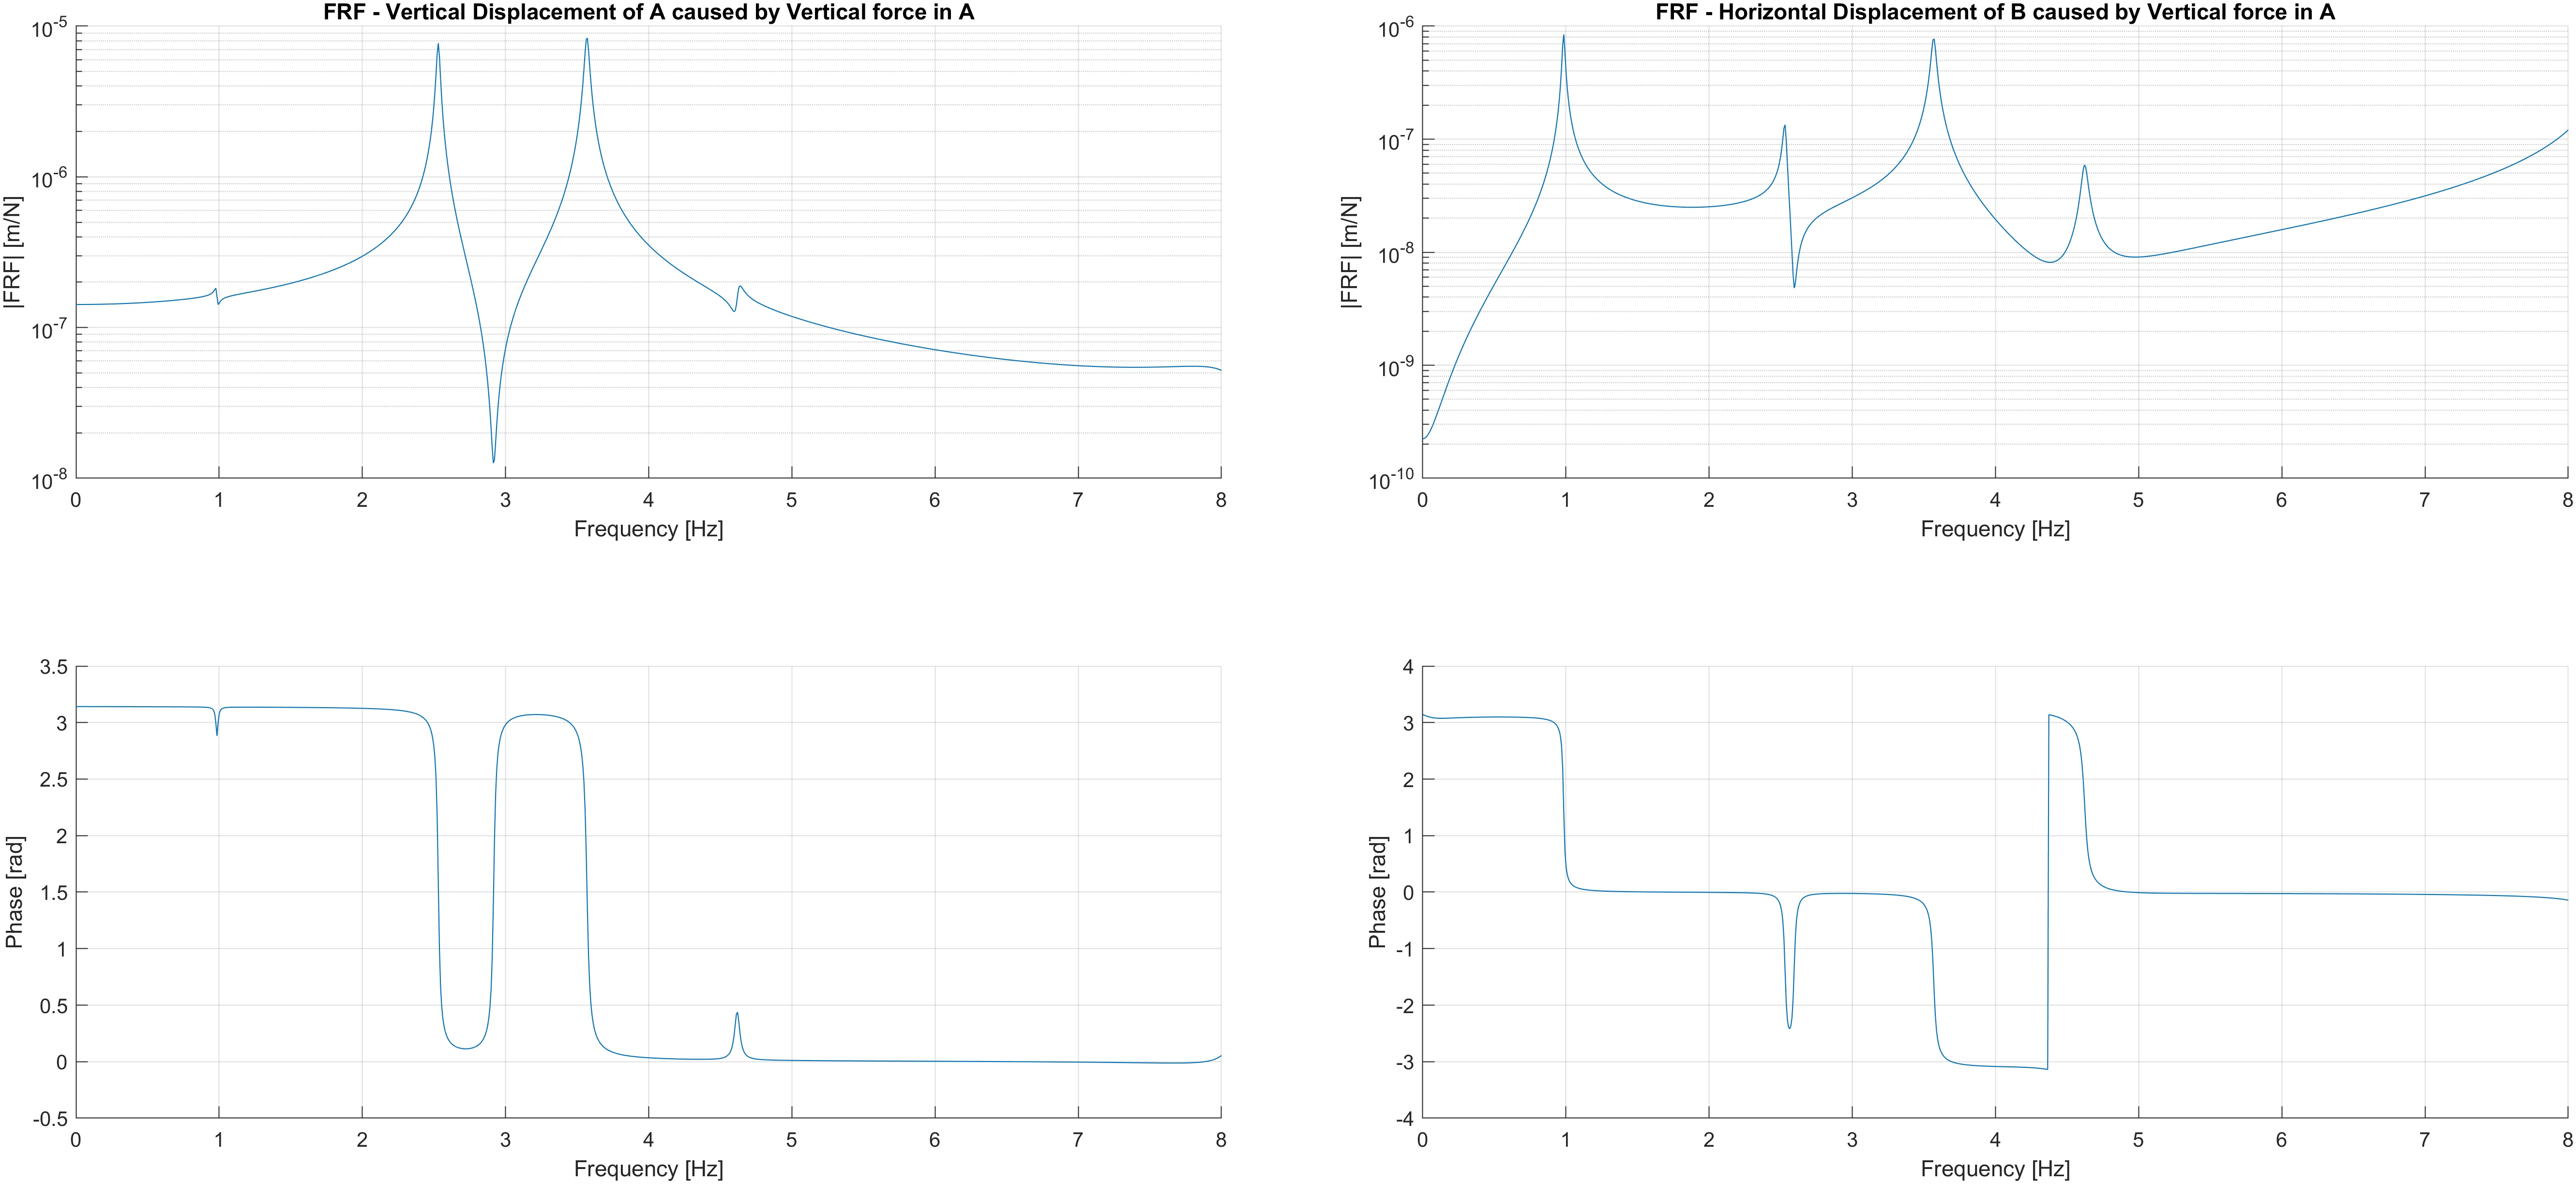
\includegraphics[width=\textwidth]{img/MATLAB/FRFs/Vertical_in_A.png}
    \caption{FRF computed using the direct method - Vertical force \textbf{A} to Vertical displacement \textbf{A} and Horizontal displacement \textbf{B}.}
    \label{fig:FRF_direct_vertical_A}
\end{figure}

From the FRFs shown in Figure \ref{fig:FRF_direct_vertical_A}, we can observe that in the considered frequency range ($0-8 [Hz]$), the vertical displacement of node \textbf{A} is more sensitive to the vertical force applied to node \textbf{A} than the horizontal displacement of node \textbf{B}.

Moreover, as expected, the resonance peaks in the FRFs correspond to the natural frequencies of the system found during modal analysis (see Section \ref{sub:modal_analysis}).

Interestingly, both FRFs exhibit an anti-resonance peak between the third and fourth natural frequencies (at $\approx 2.91 [Hz] \rightarrow 18.28 [rad/s]$), which indicates that the system's response to the excitation is minimized at that frequency.
In other words, at that specific excitation frequency, node \textbf{A} became stationary and any force applied at the corresponding frequency will not excite the system (no energy can flow from the force to the structure, null virtual work).


\subsubsection{Direct vs. Modal superposition method - Vertical force \textbf{A} to Horizontal displacement B}
\label{subsubsec:direct_vs_modal_vertical_force_A}

In this example, we compute the FRF relating the horizontal displacement of node \textbf{B} to the vertical force applied to node \textbf{A}.
We compare the results obtained using the direct method and the modal superposition method.

In order to have a significant comparison of the effect of the reduction of the number of modes considered in the analysis, we will consider only the first two mode shapes of the system in the modal superposition method ($n=2$).

\begin{figure}[H]
    \centering
    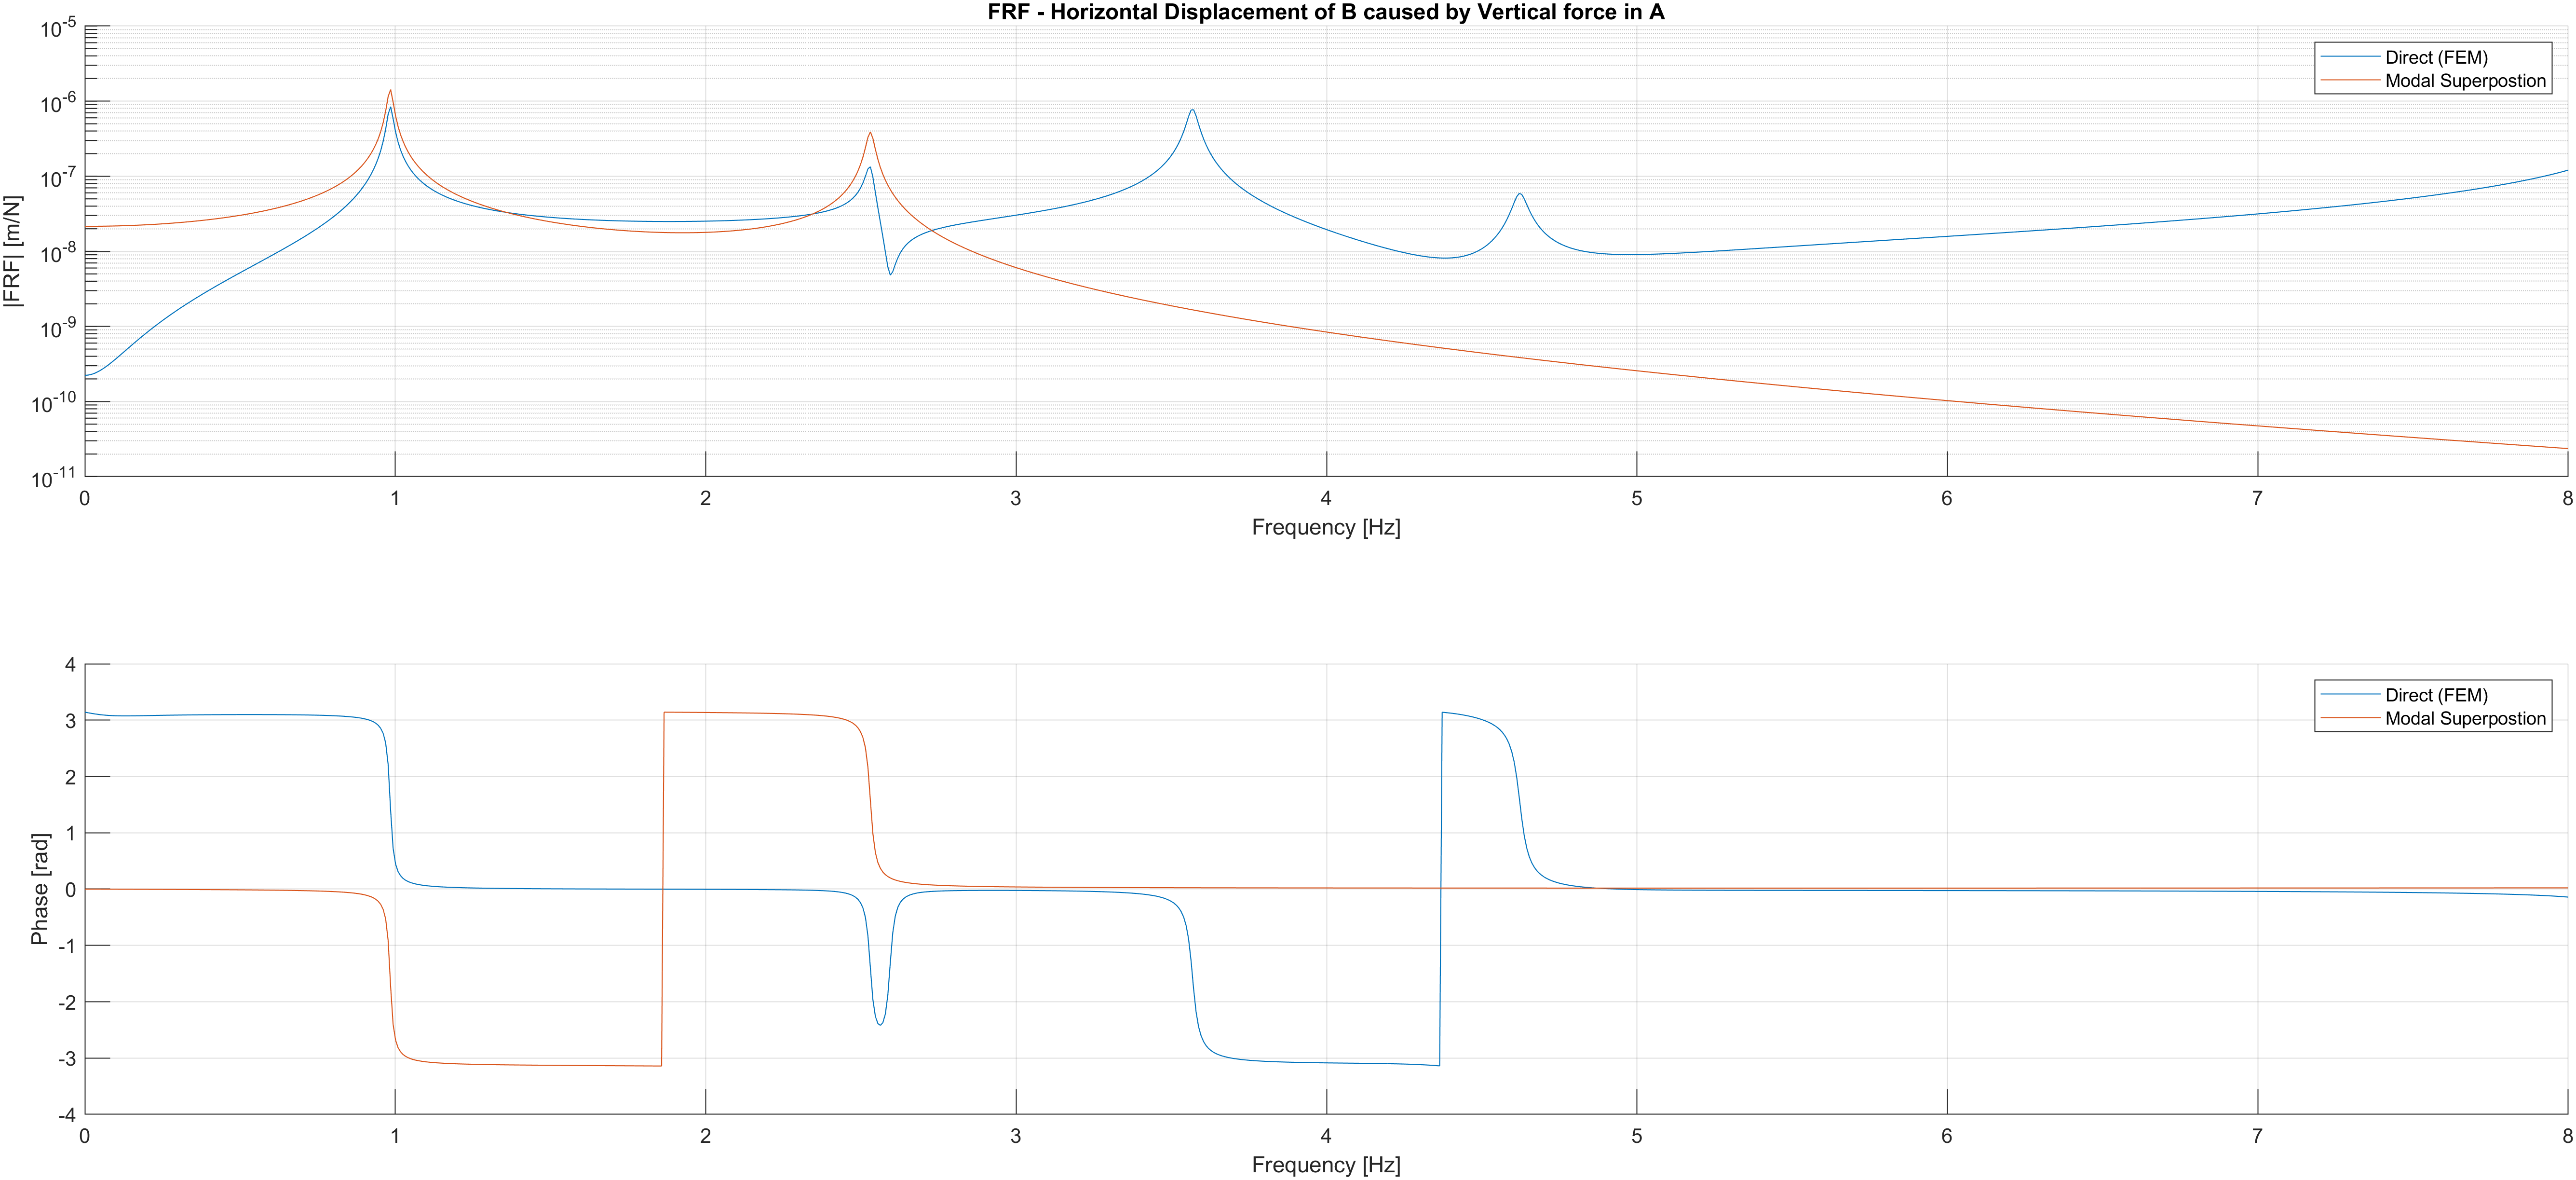
\includegraphics[width=\textwidth]{img/MATLAB/FRFs/Direct_vs_Modal.png}
    \caption{FRF computed using the direct method and modal superposition method - Vertical force \textbf{A} to Horizontal displacement \textbf{B}.}
    \label{fig:FRF_direct_vs_modal_vertical_A}
\end{figure}

From the FRFs shown in Figure \ref{fig:FRF_direct_vs_modal_vertical_A}, we can observe that the results obtained using the direct method and the modal superposition method are in good agreement only around the considered natural frequencies of the system.
As we move away from the peaks, the results start to diverge.

This behavior is expected since the modal superposition method considers only the first two mode shapes of the system, which may not capture the full dynamic behavior of the structure.
On the other hand, the direct method considers all the degrees of freedom of the system, providing a more accurate representation of the system's response to the excitation (at the cost of higher computational effort).


\subsubsection{Direct method - Vertical force \textbf{C} to Vertical reaction force \textbf{O2}}
\label{subsubsec:direct_method_vertical_force_C}

In this example, we compute the FRF relating the vertical reaction force at node \textbf{O2} to the vertical force applied to node \textbf{C}.
The FRF is computed using the direct method, considering all the degrees of freedom of the system.

\begin{figure}[H]
    \centering
    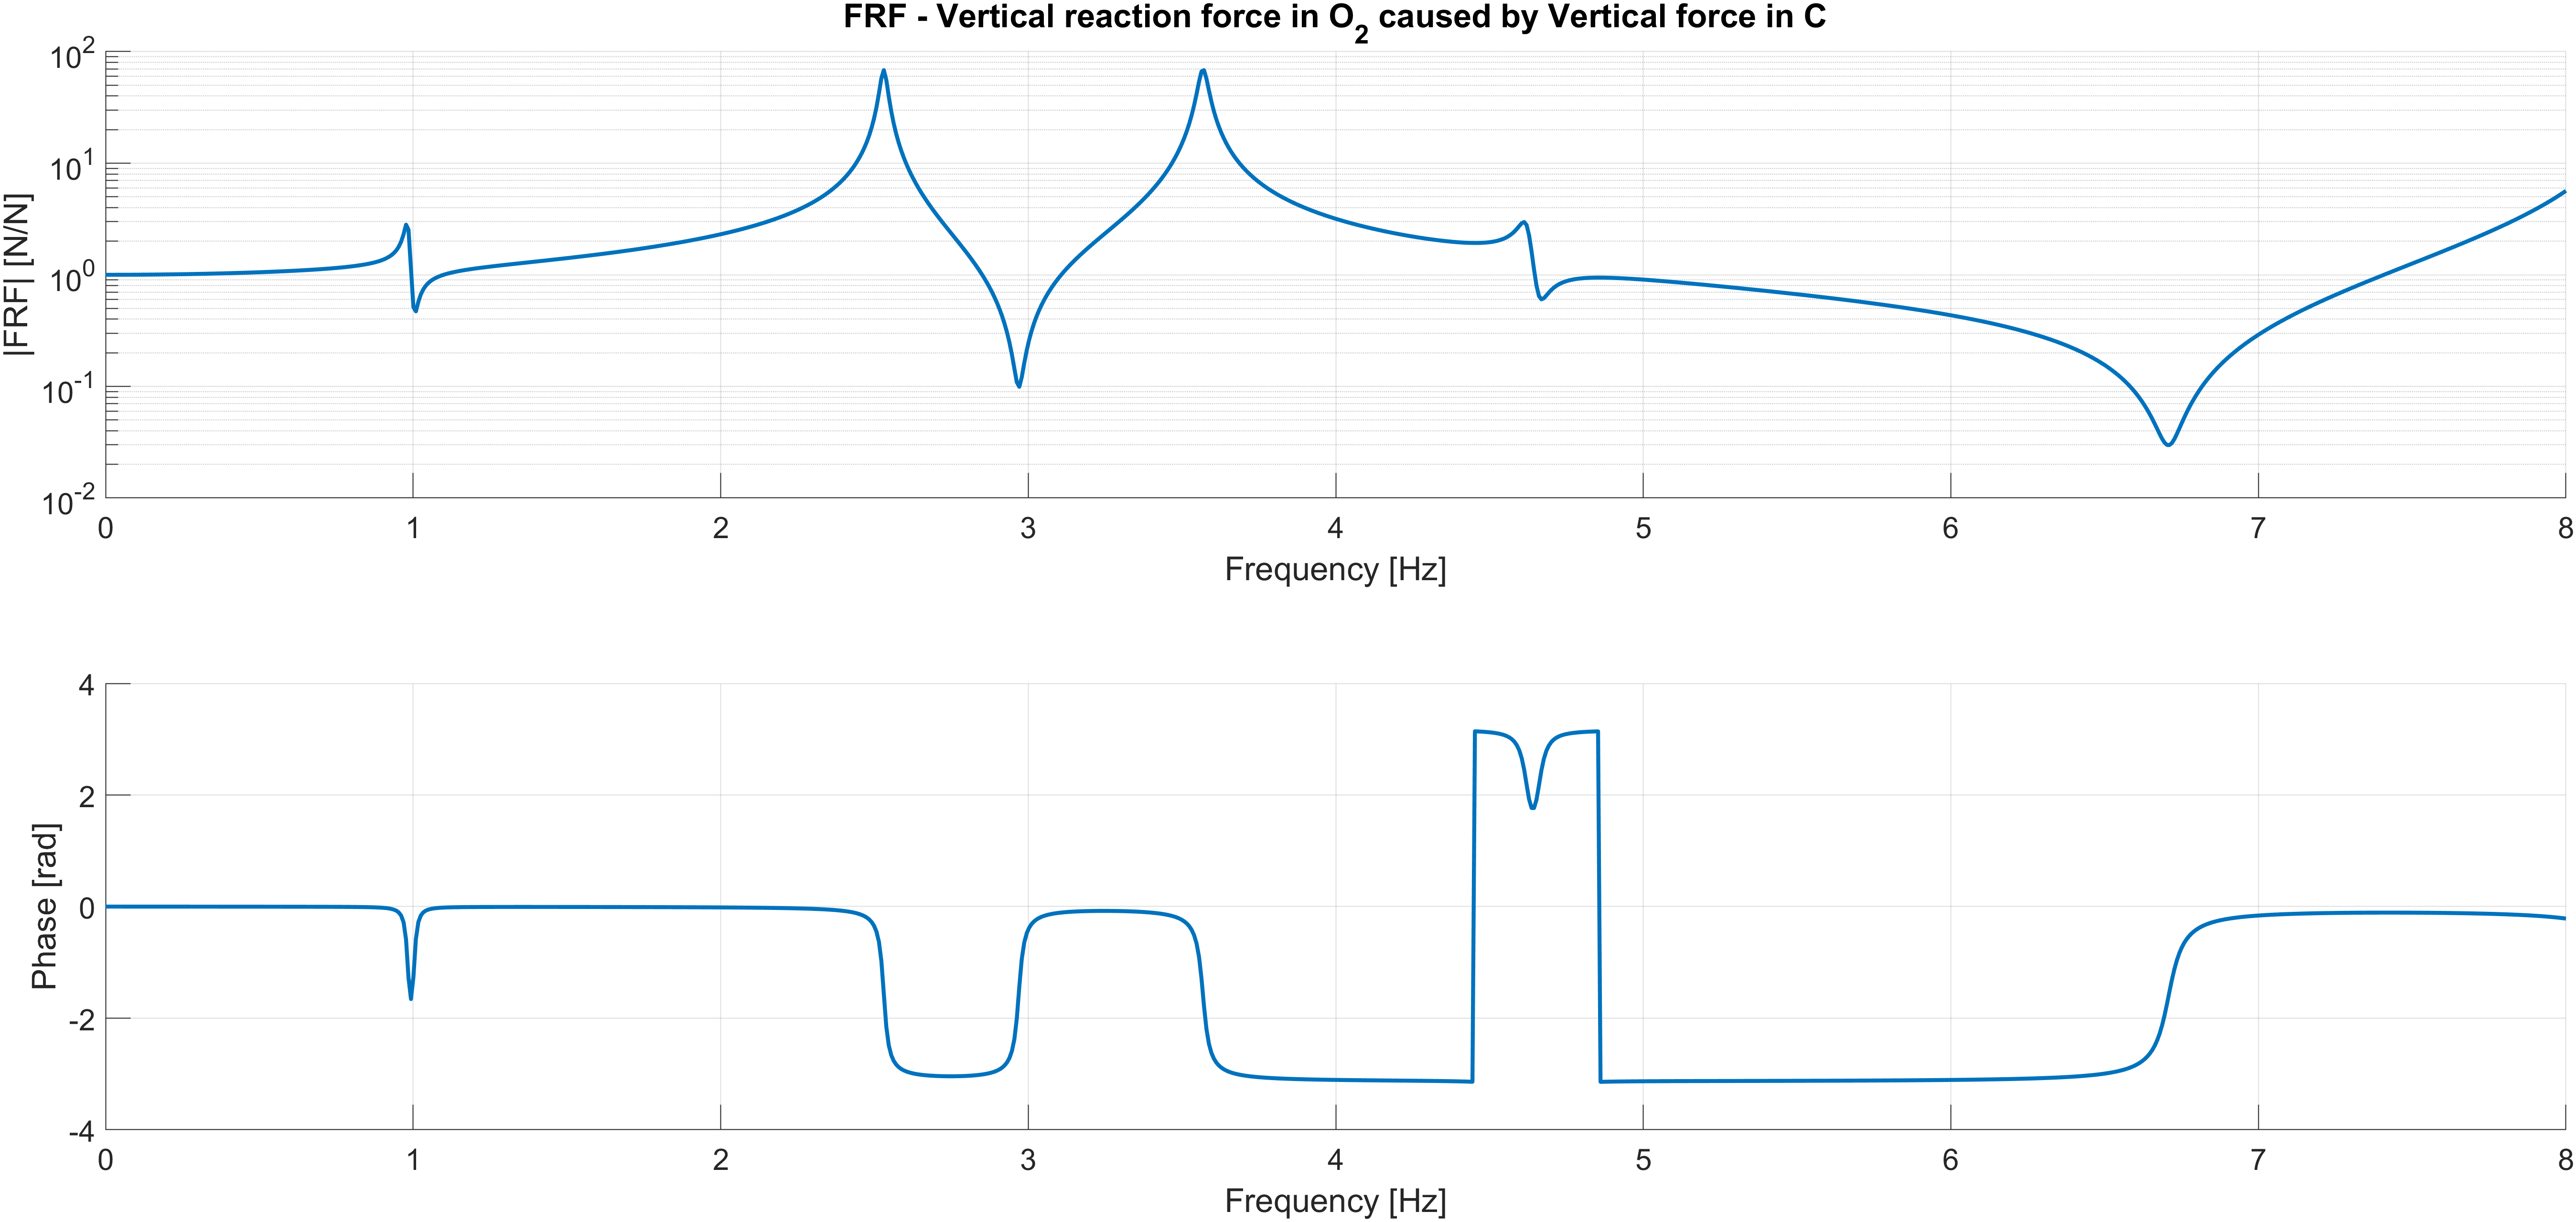
\includegraphics[width=\textwidth]{img/MATLAB/FRFs/Reaction_O2.png}
    \caption{FRF computed using the direct method - Vertical force \textbf{C} to Vertical reaction force \textbf{O2}}
    \label{fig:FRF_direct_vertical_C}
\end{figure}

Notice that reaction forces are computed in two consecutive steps: first, using the direct method the displacement in time of each node is computed obtaining the vector $\mathbf{q}(t)$, then the reaction forces are computed by substituting the displacement vector in the equation of motion relative to the constrained nodes, obtaining the reaction forces vector $\mathbf{R}(t)$.